% !TEX program = pdflatex
\documentclass[10pt,aspectratio=169]{beamer}


% Metropolis theme
\usetheme[numbering=fraction]{metropolis}
\usepackage[utf8]{inputenc}
\usepackage{CJKutf8}
\usepackage{amsmath}

\title{Conceptual Modeling}
\subtitle{ER Modeling}
\author{Michael Emmerich\\JYU Faculty of Information Technology, Finland}
\date{\today}

\usepackage{booktabs}
\usepackage[normalem]{ulem}
\usepackage{amsmath,amssymb}
\usepackage{tikz}
\usetikzlibrary{arrows.meta,positioning,shapes.geometric,shapes.misc,fit,calc,backgrounds}
\usetikzlibrary{positioning,decorations.markings}

\tikzset{
  er/entity/.style={draw, rectangle, rounded corners=2pt, minimum width=18mm, minimum height=7mm, align=center},
  er/attribute/.style={draw, ellipse, minimum width=16mm, minimum height=7mm, align=center},
  er/line/.style={draw, line width=0.5pt},
  er/isa/.style={draw, circle, inner sep=0pt, minimum size=5mm, font=\footnotesize},
  umark/.style={
    postaction={decorate},
    decoration={markings,
      mark=at position #1 with {\node[sloped,allow upside down,inner sep=0pt] {$\cup$};}
    }
  },
  childlink/.style={er/line, umark=0.85},
  totalcover/.style={er/line, double, double distance=0.8pt}
}

% -----------------------------
% TikZ styles for ER diagrams
% -----------------------------
\tikzset{
  er/entity/.style={draw, rounded corners=2pt, thick, minimum width=28mm, minimum height=9mm, align=center},
  er/weakentity/.style={er/entity, double, double distance=1.2pt},
  er/relationship/.style={draw, diamond, thick, aspect=1.8, inner sep=1.2pt, align=center, minimum width=18mm, minimum height=8mm},
  er/identrel/.style={er/relationship, double, double distance=1.2pt},
  er/attribute/.style={draw, ellipse, thick, inner sep=1.2pt, align=center, minimum width=18mm, minimum height=7mm},
  er/multival/.style={er/attribute, double, double distance=1.2pt},
  er/derived/.style={er/attribute, dashed},
  er/key/.style={er/attribute, font=\bfseries}, % underline alternative handled below
  er/isa/.style={draw, circle, thick, inner sep=0pt, minimum size=6mm, align=center},
  er/line/.style={thick},
  er/card/.style={font=\footnotesize, inner sep=1pt, fill=white},
  er/note/.style={draw, rounded corners=2pt, thick, fill=black!2, inner sep=4pt, align=left}
}

% Helper: underline attribute name (classic ER key attribute)
\newcommand{\keyattr}[1]{\underline{#1}}

% -----------------------------
% Title graphic (simple accent bar)
% -----------------------------
\newcommand{\TitleGraphic}{
\begin{tikzpicture}[remember picture,overlay]
  \fill[black!8] (current page.north west) rectangle ([yshift=-0.75cm]current page.north east);
  \fill[black!20] (current page.north west) rectangle ([yshift=-0.75cm,xshift=1.1cm]current page.north west);
\end{tikzpicture}
}
\titlegraphic{\TitleGraphic}

\begin{document}

% -----------------------------
\begin{frame}
  \titlepage
\end{frame}

% -----------------------------
\begin{frame}{Notice}
\begin{block}{Note}
The English version of the materials is work in progress. Expect bugs, typos, and other issues.
\end{block}
\end{frame}

% -----------------------------
\begin{frame}{Structure of a Database System}
\begin{itemize}
  \item A DBMS is software that enables applications and users to interact with a database.
  \item Essential expected features:
  \begin{itemize}
    \item CRUD operations: Create, Read, Update, Delete
    \item Physical data independence ($=$ can be changed without affecting other layers)
    \item Logical data independence
    \item Concurrent use
    \item Data consistency (integrity)
    \item Minimize redundancy
    \item Compatibility (systems / DBMSs)
    \item Scalability with hardware/resources
  \end{itemize}
\end{itemize}
\end{frame}

% -----------------------------
\begin{frame}{Flow of a Database Command (high-level)}
\centering
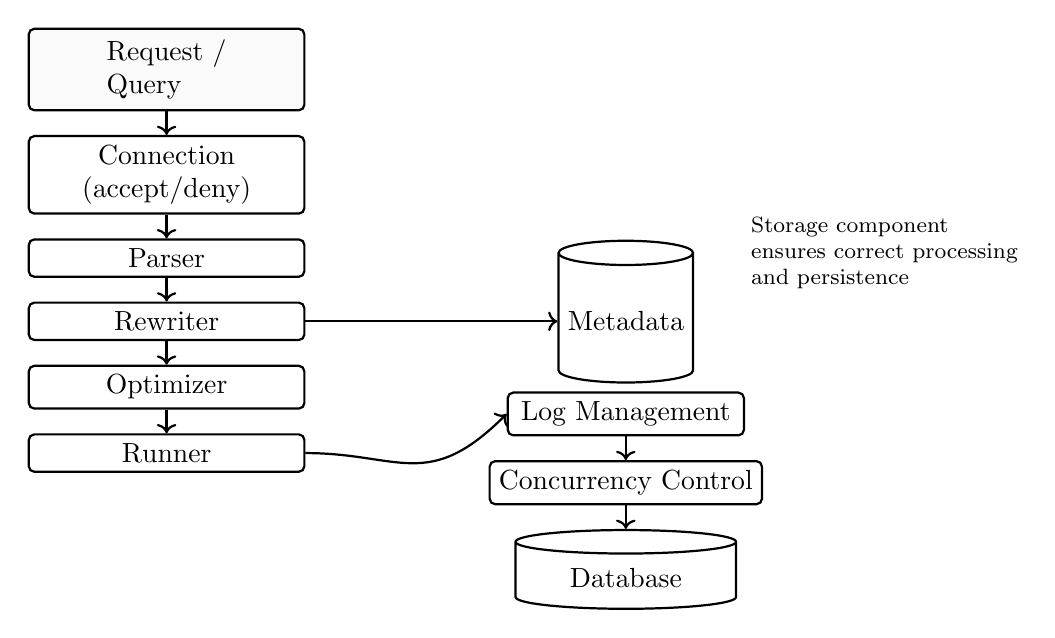
\begin{tikzpicture}[node distance=3mm and 9mm]
  % Left pipeline
  \node[er/note, minimum width=35mm] (req) {Request /\\Query};
  \node[draw, thick, rounded corners=2pt, below=of req, minimum width=35mm, align=center] (conn) {Connection\\(accept/deny)};
  \node[draw, thick, rounded corners=2pt, below=of conn, minimum width=35mm, align=center] (parser) {Parser};
  \node[draw, thick, rounded corners=2pt, below=of parser, minimum width=35mm, align=center] (rew) {Rewriter};
  \node[draw, thick, rounded corners=2pt, below=of rew, minimum width=35mm, align=center] (opt) {Optimizer};
  \node[draw, thick, rounded corners=2pt, below=of opt, minimum width=35mm, align=center] (run) {Runner};

  \draw[->, thick] (req) -- (conn);
  \draw[->, thick] (conn) -- (parser);
  \draw[->, thick] (parser) -- (rew);
  \draw[->, thick] (rew) -- (opt);
  \draw[->, thick] (opt) -- (run);

  % Storage / metadata side
  \node[draw, thick, cylinder, shape border rotate=90, aspect=0.18,
        minimum height=18mm, minimum width=16mm, right=32mm of rew] (meta) {Metadata};

  \node[draw, thick, rounded corners=2pt, below=1mm of meta, minimum width=30mm, align=center] (log) {Log Management};
  \node[draw, thick, rounded corners=2pt, below=of log, minimum width=30mm, align=center] (cc) {Concurrency Control};
  \node[draw, thick, cylinder, shape border rotate=90, aspect=0.18,
        minimum height=10mm, minimum width=28mm, below=of cc] (db) {Database};

  \draw[->, thick] (rew.east) .. controls +(12mm,0) and +(-12mm,0) .. (meta.west);
  \draw[->, thick] (run.east) .. controls +(12mm,0) and +(-10mm,-10mm) .. (log.west);
  \draw[->, thick] (log) -- (cc);
  \draw[->, thick] (cc) -- (db);

  \node[font=\footnotesize, align=left, anchor=west] at ([xshift=6mm]meta.north east)
   {Storage component\\ensures correct processing\\and persistence};
\end{tikzpicture}
\end{frame}

% -----------------------------
\begin{frame}{Conceptual Modelling}
\begin{itemize}
  \item Early stage of database design: identify domain concepts and requirements.
  \item \textbf{Data-model independent}: no commitment yet to a specific DBMS/data model.
  \item Common tool: \textbf{ER model (Entity--Relationship)}.
  \item Goal: distinguish essential data from non-essential, and make assumptions explicit.
\end{itemize}
\end{frame}




% -----------------------------
\begin{frame}{Entity Sets and Attributes}
\begin{columns}[T,onlytextwidth]
\column{0.4\textwidth}
\begin{itemize}
  \item \textbf{Entity set}: collection of similar entities (e.g., STUDENT).
  \item \textbf{Attributes}: properties (e.g., name, date of birth).
  \item ER conventions:
  \begin{itemize}
    \item Entity: rectangle
    \item Attribute: oval
    \item Attribute names often in PascalCase
  \end{itemize}
\end{itemize}

\column{0.48\textwidth}
\centering
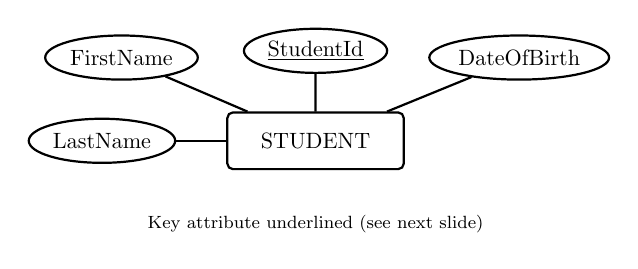
\begin{tikzpicture}[scale=0.8, transform shape,node distance=6mm and 8mm]
  \node[er/entity] (student) {STUDENT};

  \node[er/attribute, above left=of student] (fn) {FirstName};
  \node[er/attribute, left=of student] (ln) {LastName};
  \node[er/attribute, above=of student] (id) {\keyattr{StudentId}};
  \node[er/attribute, above right=of student] (dob) {DateOfBirth};

  \draw[er/line] (student) -- (fn);
  \draw[er/line] (student) -- (ln);
  \draw[er/line] (student) -- (id);
  \draw[er/line] (student) -- (dob);

  \node[font=\footnotesize, align=left, below=6mm of student] {Key attribute underlined (see next slide)};
\end{tikzpicture}
\end{columns}
\end{frame}

% -----------------------------
\begin{frame}{Key Attribute}
\begin{itemize}
  \item Entities in an entity set must be \textbf{uniquely identifiable}.
  \item A \textbf{key attribute} (or key attribute set, e.g. birthdate and Name) uniquely identifies each entity.
  \item Key attributes \textbf{cannot be null} and are typically \textbf{underlined}.
  \item Example: student name is not unique; a StudentId (or national student number) is.
  \item Safe-guarding the uniqueness of keys can be a problem in large-scale databases. 
  \item[] $\Rightarrow$ Choose keys wisely. Make sure they are easy to manage.
  \item[] \textit{For instance}, do not just use names, as there might be duplicates. (E.g., \texttt{Athens} is a city in Greece and in the USA, \texttt{George Clinton} (Funk Musician and Founding Father)).
\end{itemize}
\end{frame}

% -----------------------------
\begin{frame}{Composite, Derived, Multivalued Attributes}
\begin{columns}[T,onlytextwidth]
\column{0.50\textwidth}

\textbf{Composite attribute (Address)}:
\vspace{0.5cm}

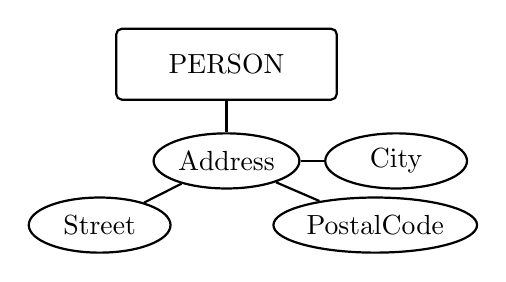
\begin{tikzpicture}[node distance=3mm and 3mm]
  \node[er/entity] (person) {PERSON};
  \node[er/attribute, below=4mm of person] (addr) {Address};
  \node[er/attribute, below left=of addr] (street) {Street};
  \node[er/attribute, right=of addr] (city) {City};
  \node[er/attribute, below right=of addr] (zip) {PostalCode};

  \draw[er/line] (person) -- (addr);
  \draw[er/line] (addr) -- (street);
  \draw[er/line] (addr) -- (city);
  \draw[er/line] (addr) -- (zip);
\end{tikzpicture}

\column{0.50\textwidth}
\textbf{Derived and multivalued}:
\vspace{0.5cm}

\begin{tikzpicture}[node distance=6mm and 10mm]
  \node[er/entity] (student) {STUDENT};
  \node[er/derived, above=of student] (age) {Age};
  \node[er/multival, right=14mm of student] (phone) {Phone};
  \node[er/multival, below=of phone] (email) {Email};
  \node[er/attribute, below=4mm of person] (dbirth) {DateOfBirth};

  \draw[er/line] (student) -- (age);
  \draw[er/line] (student) -- (phone);
  \draw[er/line] (student) -- (email);
  \draw[er/line] (student) -- (dbirth);
\end{tikzpicture}

\vspace{2mm}
\begin{itemize}\footnotesize
  \item Derived: computed (store only if needed)
  \item Multivalued: multiple values per entity
\end{itemize}
\end{columns}
\end{frame}

% -----------------------------
\begin{frame}{Relationship Sets}
\begin{columns}[T,onlytextwidth]
\column{0.50\textwidth}
\begin{itemize}
  \item Relationship set connects entity sets. 
  \item May have attributes of its own (e.g., completion date).
  \item It can be seen as a set of tuples with components taken from the entity sets and the domain of the attributes, e.g. $(s, c, d)$ with $s \in STUDENT$, $c \in COURSE, d \in Date$. Here $Date$ is the attribute domain of dates.
  \item Often named with a \textbf{verb phrase} (e.g., Completes).
\end{itemize}

\column{0.50\textwidth}
\centering
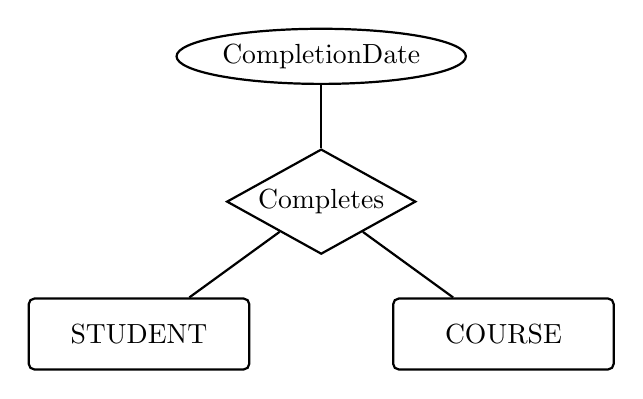
\begin{tikzpicture}[node distance=8mm and 10mm]
  \node[er/entity] (stud) {STUDENT};
  \node[er/entity, right=18mm of stud] (course) {COURSE};
  \node[er/relationship, above=10mm of $(stud)!0.5!(course)$] (comp) {Completes};
  \node[er/attribute, above=of comp] (date) {CompletionDate};

  \draw[er/line] (stud) -- (comp);
  \draw[er/line] (course) -- (comp);
  \draw[er/line] (comp) -- (date);
\end{tikzpicture}
\end{columns}
\end{frame}

% -----------------------------
\begin{frame}{Degree of a Relationship}
\begin{columns}[T,onlytextwidth]
\column{0.50\textwidth}
\textbf{Unary relationship} \\(e.g., Employee supervises Employee):
\medskip

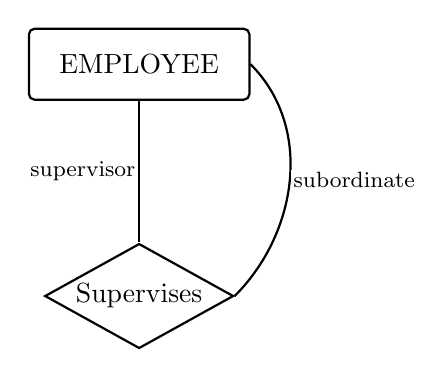
\begin{tikzpicture}[node distance=8mm and 10mm]
  \node[er/entity] (emp) {EMPLOYEE};
  \node[er/relationship, below=18mm of emp] (sup) {Supervises};

  % first participation + role label
  \draw[er/line] (emp) -- (sup)
    node[midway, left, er/card] {supervisor};

  % second participation (recursive) + role label
  \draw[er/line]
    (emp.east) .. controls +(8mm,-8mm) and +(8mm,8mm) .. (sup.east)
    node[midway, right, er/card] {subordinate};
\end{tikzpicture}
\begin{itemize}
    \item You can assign roles to the links, e.g., "supervisor" and "subordinate"
\end{itemize}

\column{0.50\textwidth}
\textbf{Ternary relationship} (e.g., Teacher grades Student in Course):
\vspace{0.5cm}

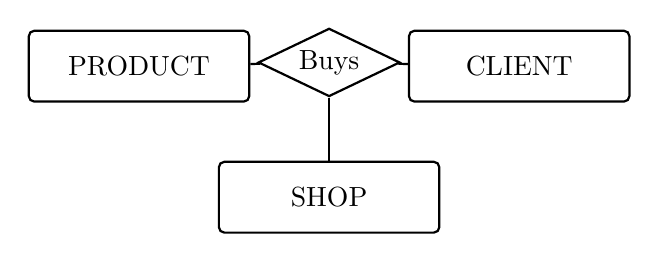
\begin{tikzpicture}[node distance=7mm and 12mm]
  \node[er/entity] (teacher) {PRODUCT};
  \node[er/entity, right=20mm of teacher] (student) {CLIENT};
  \node[er/entity, below=12mm of $(teacher)!0.5!(student)$] (course) {SHOP};

  \node[er/relationship, above=8mm of course] (grade) {Buys};

  \draw[er/line] (teacher) -- (grade);
  \draw[er/line] (student) -- (grade);
  \draw[er/line] (course) -- (grade);
\end{tikzpicture}
\begin{itemize}
    \item Not equivalent to 3 binary relationships: Product was bought in a shop, Shop has product, Client bought product.
    \item Alternative: Central 'contract' entity could be used that connects the three entities by binary relations. 
\end{itemize}
\end{columns}
\end{frame}

% -----------------------------
\begin{frame}{Cardinality: Min/Max Participation}
\begin{itemize}
  \item Cardinality expresses \textbf{how many} entities can/must participate.
  \item Use \textbf{min} (0 or 1) and \textbf{max} (1 or N) near each side.
  \item Example: \textbf{PERSON owns CAR}
  \begin{itemize}
    \item A person may own 0..N cars
    \item A car must have exactly 1 owner (1..1)
    \item A team has exactly 11 players 
    \item A player can play at most in one team
  \end{itemize}
\end{itemize}

\centering
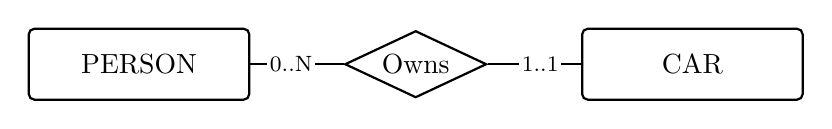
\begin{tikzpicture}[node distance=8mm and 18mm]
  \node[er/entity] (person) {PERSON};
  \node[er/entity, right=42mm of person] (car) {CAR};
  \node[er/relationship] (owns) at ($(person)!0.5!(car)$) {Owns};

  \draw[er/line] (person) -- (owns);
  \draw[er/line] (car) -- (owns);

  \node[er/card] at ($(person)!0.55!(owns)$) {0..N};
  \node[er/card] at ($(car)!0.55!(owns)$) {1..1};
\end{tikzpicture}
\medskip

\begin{tikzpicture}[node distance=8mm and 18mm]
  \node[er/entity] (player) {PLAYER};
  \node[er/entity, right=42mm of player] (team) {TEAM};
  \node[er/relationship] (playsIn) at ($(person)!0.5!(team)$) {playsIn};
  \draw[er/line] (player) -- (playsIn);
  \draw[er/line] (team) -- (playsIn);

  \node[er/card] at ($(team)!0.55!(playsIn)$) {11..11};
  \node[er/card] at ($(player)!0.55!(playsIn)$) {0..1};
\end{tikzpicture}
\end{frame}

% ------------------------------


% -----------------------------
\begin{frame}{Different Cardinality Notations}
\begin{itemize}
  \item Several notations exist (Chen, UML, Crow's foot / Hoffer--Prescott--McFadden).
  \item Examples: see course materials on TIM
  \item Pick one and be consistent within a course/project.
  \item Under the hood, most notations communicate:
  \begin{itemize}
    \item minimum participation (0 or 1)
    \item maximum participation (1 or many)
  \end{itemize}
  \item In mathematics: many-to-one, one-to-one, one-to-one correspondence.
  \item \textbf{Useful Question to Determine Cardinality (M..N):} 
  \item[] \textit{"How many times must (M) and can (N) a entity from the entity set participate in the relationship set?"}
\end{itemize}
\end{frame}

% -----------------------------
\begin{frame}{Weak Entity Set and Identifying Relationship}
\begin{itemize}
  \item A \textbf{weak entity} cannot be uniquely identified by its own attributes alone.
  \item It is identified through an \textbf{identifying relationship} with a strong entity.
  \item Rule of thumb: max cardinality of weak entity in identifying relationship is often 1.
\end{itemize}

\centering
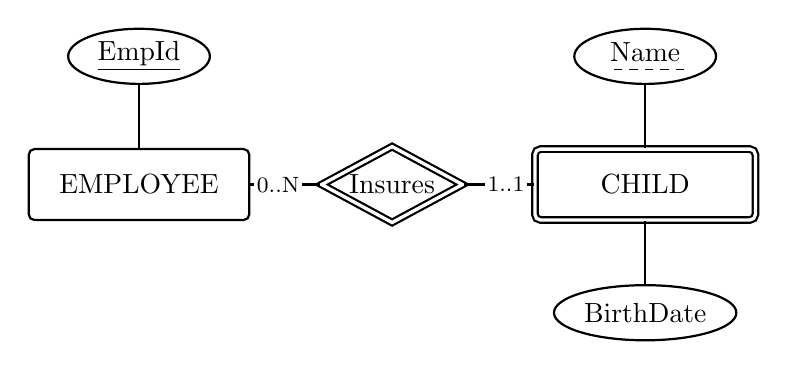
\begin{tikzpicture}[node distance=8mm and 12mm]
  \node[er/entity] (company) {EMPLOYEE};
  \node[er/weakentity, right=36mm of company] (dept) {CHILD};

  \node[er/identrel] (owns) at ($(company)!0.5!(dept)$) {Insures};

  \node[er/attribute, above=of company] (cid) {\keyattr{EmpId}};
  \node[er/attribute, above=of dept] (did) {\dashuline{Name}};
  \node[er/attribute, below=of dept] (dname) {BirthDate};

  \draw[er/line] (company) -- (owns);
  \draw[er/line] (dept) -- (owns);

  \draw[er/line] (company) -- (cid);
  \draw[er/line] (dept) -- (did);
  \draw[er/line] (dept) -- (dname);

  \node[er/card] at ($(company)!0.55!(owns)$) {0..N};
  \node[er/card] at ($(dept)!0.55!(owns)$) {1..1};
\end{tikzpicture}
\begin{itemize}
    \item Used when a list of entities (e.g. children) is attached to an Entity (e.g. employee). When owner entity is removed from database so are the dependents. 
    \item Why? $\Rightarrow$ Key management becomes easier. Data consistency is enforced. 
\end{itemize}
\end{frame}

% -----------------------------
\begin{frame}{Abstraction Structures (EER): Generalization}
\begin{columns}[T,onlytextwidth]
\column{0.48\textwidth}
\begin{itemize}
  \item Use \textbf{E}xtended ER (EER) to model inheritance-like structures.
  \item A \textbf{super-entity} has shared attributes.
  \item \textbf{sub-entities} specialize it (e.g., STUDENT, STAFF).
  \item Subtypes can have specific relationships (e.g. STAFF has CONTRACT)
  \item Disjoint vs overlapping; total vs partial.
  \begin{itemize}
  \item Supertype: \textbf{PERSON}; subtypes: \textbf{STUDENT}, \textbf{STAFF} (U-marks = children; 1/2 lines = partial/total coverage).
  \item Circle label: \textbf{d} = disjoint, \textbf{o} = overlapping.
\end{itemize}

\end{itemize}

\column{0.52\textwidth}
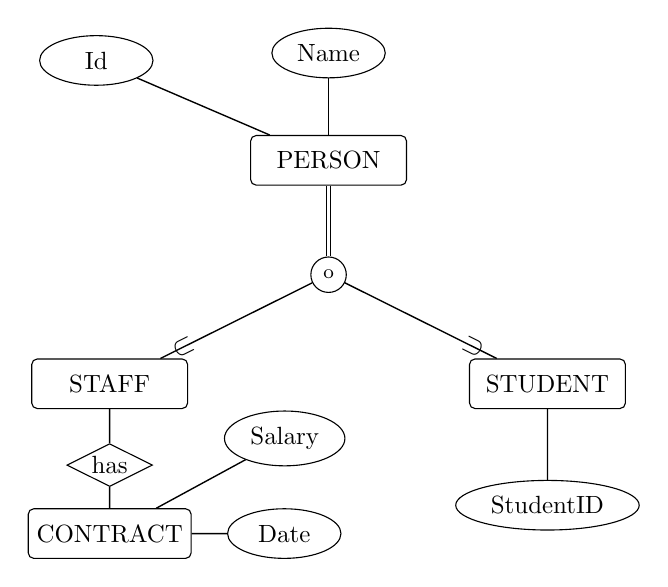
\begin{tikzpicture}[
  scale=0.9, transform shape,
  node distance=8mm and 16mm,
  entity/.style={draw, rectangle, rounded corners=2pt, minimum width=22mm, minimum height=7mm, align=center},
  attr/.style={draw, ellipse, minimum width=16mm, minimum height=7mm, align=center},
  rel/.style={draw, diamond, aspect=2, inner sep=1pt, align=center},
  line/.style={draw, line width=0.5pt},
  isa/.style={draw, circle, inner sep=0pt, minimum size=5mm, font=\footnotesize}
]

% --- Supertype PERSON + attributes ---
\node[entity] (person) {PERSON};
\node[attr, above left=of person] (pid) {Id};
\node[attr, above=of person] (name) {Name};
\draw[line] (person) -- (pid);
\draw[line] (person) -- (name);

% --- ISA (overlapping) ---
\node[isa, below=10mm of person] (isa) {o};

\node[entity, below left=10mm and 18mm of isa] (staff) {STAFF};
\node[entity, below right=10mm and 18mm of isa] (stud) {STUDENT};

% total coverage (double line)
\draw[line, double, double distance=0.8pt] (person) -- (isa);

% child links with rotated U
\draw[line,
  postaction={decorate},
  decoration={markings,
    mark=at position 0.85 with {
      \node[sloped,allow upside down,inner sep=0pt,rotate=90] {$\cup$};
    }
  }
] (isa) -- (staff);

\draw[line,
  postaction={decorate},
  decoration={markings,
    mark=at position 0.85 with {
      \node[sloped,allow upside down,inner sep=0pt,rotate=90] {$\cup$};
    }
  }
] (isa) -- (stud);

% --- STUDENT attribute: StudentID ---
\node[attr, below=10mm of stud] (sid) {StudentID};
\draw[line] (stud) -- (sid);

% --- CONTRACT entity + attributes ---
\node[entity, below=14mm of staff] (contract) {CONTRACT};
\node[attr, above right=10mm of contract] (salary) {Salary};
\node[attr, right=5mm of contract] (cdate) {Date};
\draw[line] (contract) -- (salary);
\draw[line] (contract) -- (cdate);

% --- Relationship HAS between STAFF and CONTRACT ---
\node[rel, above=3mm of contract] (has) {has};
\draw[line] (staff) -- (has);
\draw[line] (has) -- (contract);

\end{tikzpicture}

\end{columns}
\end{frame}


% -----------------------------

% Put this OUTSIDE the frame (preamble or before this frame)
\newcommand{\childlinkU}[4]{%
  \draw[link,->] (#1) to[bend left=#3]
    node[pos=0.82, sloped, allow upside down, inner sep=0pt, rotate=#4] {$\cup$}
  (#2);
}

\begin{frame}{Disjoint vs Overlapping; Total vs Partial}

\begin{itemize}
  \item \textbf{Disjoint} (d): an entity belongs to \emph{at most one} sub-entity set.
  \item \textbf{Overlapping} (o): an entity may belong to \emph{multiple} sub-entity sets.
  \item \textbf{Total}: the entity set is the set union of all sub-entity sets. Otherwise: partial. Use $||$ to indicate totality.
\end{itemize}

\centering
\hspace{-0.5cm}
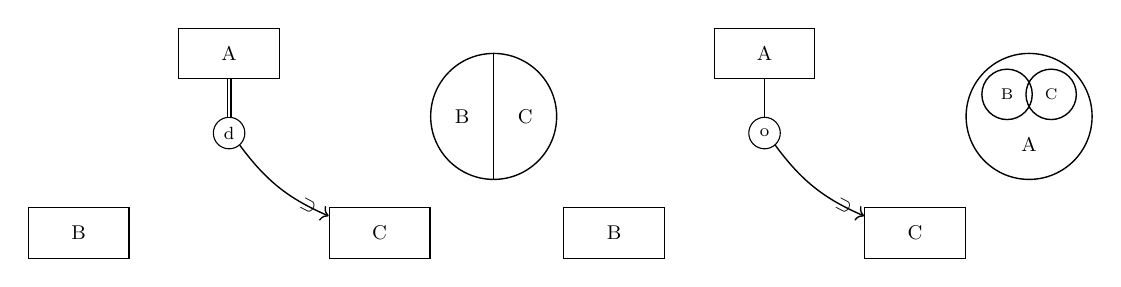
\begin{tikzpicture}[scale=0.8, transform shape,
  entity/.style={draw, rectangle, minimum width=16mm, minimum height=8mm, align=center},
  isa/.style={draw, circle, inner sep=0pt, minimum size=5mm, font=\footnotesize},
  link/.style={draw, line width=0.5pt},
  cover/.style={link, double, double distance=0.8pt}, % total cover
  every node/.style={font=\small}
]

% ==================== LEFT GROUP ====================
\begin{scope}[xshift=0mm]
  \node[entity] (A1) {A};
  \node[isa, below=6mm of A1] (d1) {d};
  \node[entity, below left=10mm and 14mm of d1] (B1) {B};
  \node[entity, below right=10mm and 14mm of d1] (C1) {C};

  % total cover (double line); for partial cover use: \draw[link] (A1) -- (d1);
  \draw[cover] (A1) -- (d1);

  % child links with U markers (left/right)
  \childlinkU{d1}{B1}{15}{90}
  \draw[link,->] (d1) to[bend right=15]
    node[pos=0.82, sloped, allow upside down, inner sep=0pt, rotate=90] {$\cup$}
  (C1);

  % small circle showing B | C
  \begin{scope}[xshift=42mm, yshift=-10mm]
    \draw[link] (0,0) circle (10mm);
    \draw[link] (0,-10mm) -- (0,10mm);
    \node at (-5mm,0) {B};
    \node at ( 5mm,0) {C};
  \end{scope}
\end{scope}

% ==================== RIGHT GROUP ====================
\begin{scope}[xshift=85mm]
  \node[entity] (A2) {A};
  \node[isa, below=6mm of A2] (d2) {o};
  \node[entity, below left=10mm and 14mm of d2] (B2) {B};
  \node[entity, below right=10mm and 14mm of d2] (C2) {C};

  % total cover (double line); for partial cover use: \draw[link] (A2) -- (d2);
  \draw (A2) -- (d2);

  % child links with U markers (left/right)
  \childlinkU{d2}{B2}{15}{90}
  \draw[link,->] (d2) to[bend right=15]
    node[pos=0.82, sloped, allow upside down, inner sep=0pt, rotate=90] {$\cup$}
  (C2);
\end{scope}

% small circle with B,C inside and A below (for the RIGHT group)
\begin{scope}[xshift=127mm, yshift=-10mm]
  \draw[link] (0,0) circle (10mm);
  \draw[link] (-3.5mm,3.5mm) circle (4mm);
  \draw[link] ( 3.5mm,3.5mm) circle (4mm);
  \node at (-3.5mm,3.5mm) {\scriptsize B};
  \node at ( 3.5mm,3.5mm) {\scriptsize C};
  \node at (0,-4.5mm) {A};
\end{scope}

\end{tikzpicture}

\end{frame}


% -----------------------------
\begin{frame}{Aggregation (Conceptual Grouping)}
\begin{itemize}
  \item Aggregation treats a relationship + participating entities as a higher-level unit.
  \item Useful when you need to relate something to an \emph{interaction}, not just entities.
\end{itemize}

\centering
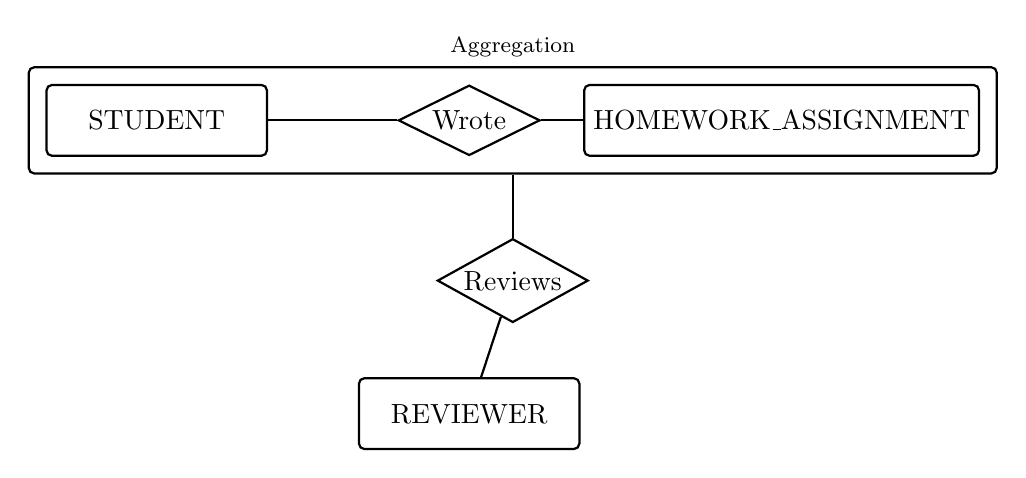
\begin{tikzpicture}[node distance=8mm and 12mm]
  % Base entities and relationship
  \node[er/entity] (emp) {STUDENT};
  \node[er/entity, right=40mm of emp] (office) {HOMEWORK\_ASSIGNMENT};
  \node[er/relationship] (works) at ($(emp)!0.5!(office)$) {Wrote};

  \draw[er/line] (emp) -- (works);
  \draw[er/line] (office) -- (works);

  % Aggregation box around (emp-works-office)
  \node[draw, thick, rounded corners=2pt, fit=(emp)(works)(office), inner sep=6pt, label={[font=\footnotesize]above:Aggregation}] (agg) {};

  % Customer relates to the aggregated unit (example)
  \node[er/entity, below=28mm of works] (reviewer) {REVIEWER};
  \node[er/relationship, below=8mm of agg] (reviews) {Reviews};

  \draw[er/line] (reviewer) -- (reviews);
  \draw[er/line] (reviews) -- ($(agg.south)$);
\end{tikzpicture}
\end{frame}

% -----------------------------
\begin{frame}{Phases of Conceptual Modelling}
\begin{enumerate}
  \item \textbf{Draw requirements} (domain, needs, constraints). Avoid modeling irrelevant details.
  \item \textbf{Identify entity sets} from recurring concepts (nouns).
  \item \textbf{Identify relationship sets and cardinalities} from relevant verbs.
  \item \textbf{Identify attributes}
  \begin{itemize}
    \item choose key attributes
    \item mark special attributes (multivalued, derived, composite)
  \end{itemize}
  \item \textbf{Iterate and refactor}
  \begin{itemize}
    \item add missing entities/relationships
    \item rename for clarity
    \item check cardinalities from the domain perspective
    \item use abstraction if it improves understanding
  \end{itemize}
\end{enumerate}
\end{frame}

% -----------------------------
\begin{frame}{Worked Mini-Example (from a text description)}
\small
\textbf{Domain snippet (example):}
\begin{itemize}
  \item Customers: customerId, name, address
  \item Products: productId, name, price
  \item Orders: orderNumber
  \item An order concerns multiple products (with quantities)
\end{itemize}

\vspace{1mm}
\centering
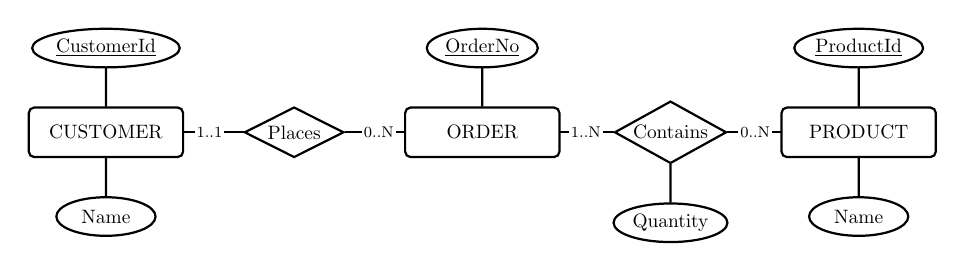
\begin{tikzpicture}[scale=0.7, transform shape,node distance=7mm and 14mm]
  \node[er/entity] (cust) {CUSTOMER};
  \node[er/entity, right=40mm of cust] (order) {ORDER};
  \node[er/entity, right=40mm of order] (prod) {PRODUCT};

  \node[er/relationship] (places) at ($(cust)!0.5!(order)$) {Places};
  \node[er/relationship] (contains) at ($(order)!0.5!(prod)$) {Contains};

  \node[er/attribute, above=of cust] (cid) {\keyattr{CustomerId}};
  \node[er/attribute, below=of cust] (cname) {Name};

  \node[er/attribute, above=of order] (onum) {\keyattr{OrderNo}};

  \node[er/attribute, above=of prod] (pid) {\keyattr{ProductId}};
  \node[er/attribute, below=of prod] (pname) {Name};
  \node[er/attribute, below=of contains] (qty) {Quantity};

  \draw[er/line] (cust)--(places);
  \draw[er/line] (order)--(places);

  \draw[er/line] (order)--(contains);
  \draw[er/line] (prod)--(contains);
  \draw[er/line] (contains)--(qty);

  \draw[er/line] (cust)--(cid);
  \draw[er/line] (cust)--(cname);
  \draw[er/line] (order)--(onum);
  \draw[er/line] (prod)--(pid);
  \draw[er/line] (prod)--(pname);

  % Example cardinalities (illustrative)
  \node[er/card] at ($(cust)!0.55!(places)$) {1..1};
  \node[er/card] at ($(order)!0.55!(places)$) {0..N};

  \node[er/card] at ($(order)!0.55!(contains)$) {1..N};
  \node[er/card] at ($(prod)!0.55!(contains)$) {0..N};
\end{tikzpicture}
\end{frame}

% -----------------------------
\begin{frame}{Checklist When Finalizing an ER Model}
\begin{itemize}
  \item Are entities and relationships named clearly from the domain perspective?
  \item Are key attributes chosen and justified? Any nullability issues?
  \item Do cardinalities reflect the real rules (min and max)?
  \item Any attributes that are better modeled as entities (e.g., repeating groups)?
  \item Any derived attributes that should not be stored?
  \item Would EER abstractions reduce duplication and improve clarity?
\end{itemize}
\end{frame}

% -----------------------------
\begin{frame}{Summary}
\begin{itemize}
  \item Conceptual modeling is data-model independent and focuses on domain meaning.
  \item ER basics: entities, attributes, relationships, keys.
  \item Important refinements: cardinalities, weak entities, EER abstractions, aggregation.
  \item Simple \textit{cardinality constraints} and \textit{inheritance constraints} can be modelled
  \item \textbf{Praxis tip:} Write down complex (hard-to-express) constraints beneath the diagram so they are not forgotten in later modeling steps.
  \item Iterate: refine names, constraints, and assumptions until the model is stable.
\end{itemize}
\end{frame}

\begin{frame}{ER Model (Chen): a short history + a language analogy}
\begin{columns}[T,onlytextwidth]
\small
  \begin{column}{0.58\textwidth}
    \textbf{Peter Pin-Shan Chen} proposed 
    \begin{itemize}
      \item Proposed the \textbf{Entity–Relationship (ER) model} as a high-level, implementation-independent database design method.
      \item Goal: separate \textbf{conceptual modeling} (meaning) from \textbf{logical/physical design} (tables, indexes, storage).
    \end{itemize}

    \vspace{0.4em}
    \textbf{Key milestones}
    \begin{itemize}
      \item \textbf{1976}: Chen publishes ``The Entity--Relationship Model Toward a Unified View of Data'' (introduces entities, relationships, attributes).
      \item \textbf{Late 1970s--1980s}: ER diagrams adopted in practice; extended ER (EER) adds specialization/generalization, weak entities, richer constraints.
      \item \textbf{1990s--today}: ER ideas live on in UML class diagrams and modern conceptual schema design.
    \end{itemize}
  \end{column}

  \begin{column}{0.42\textwidth}
    \textbf{Analogy to Chinese character composition}
    \vspace{0.3em}

    In Chinese, simple parts combine to express meaning:\\
\begin{CJK}{UTF8}{gbsn} % or another available CJK font
% ... your frame with 日 月 明 ...
      \text{日 (sun)} $+$ \text{月 (moon)}  $\rightarrow$ \text{明 (bright)}
\end{CJK}
    
    (often explained as ``bright objects'') 

    \vspace{0.6em}
    \textbf{Parallel to ER modeling}
    \begin{itemize}
      \item \textbf{Entities} $\approx$ semantic building blocks (``things'')
      \item \textbf{Relationships} $\approx$ how blocks combine (structure)
      \item \textbf{Attributes/constraints} $\approx$ additional semantics
    \end{itemize}
    \vspace{0.4em}
  \end{column}
\end{columns}
\end{frame}

\end{document}
